\glspl{llm} have emerged as a transformative innovation in \gls{nlp}, leveraging \gls{dl} techniques to understand, generate, and manipulate human language with unprecedented accuracy.
Fig.~\ref{fig:llms-over-the-years} shows the increasing trend in the number of \glspl{llm} releases and the names of some significant \glspl{llm} proposed from 2019 to 2024.

\begin{figure}[htbp]
    \centering
 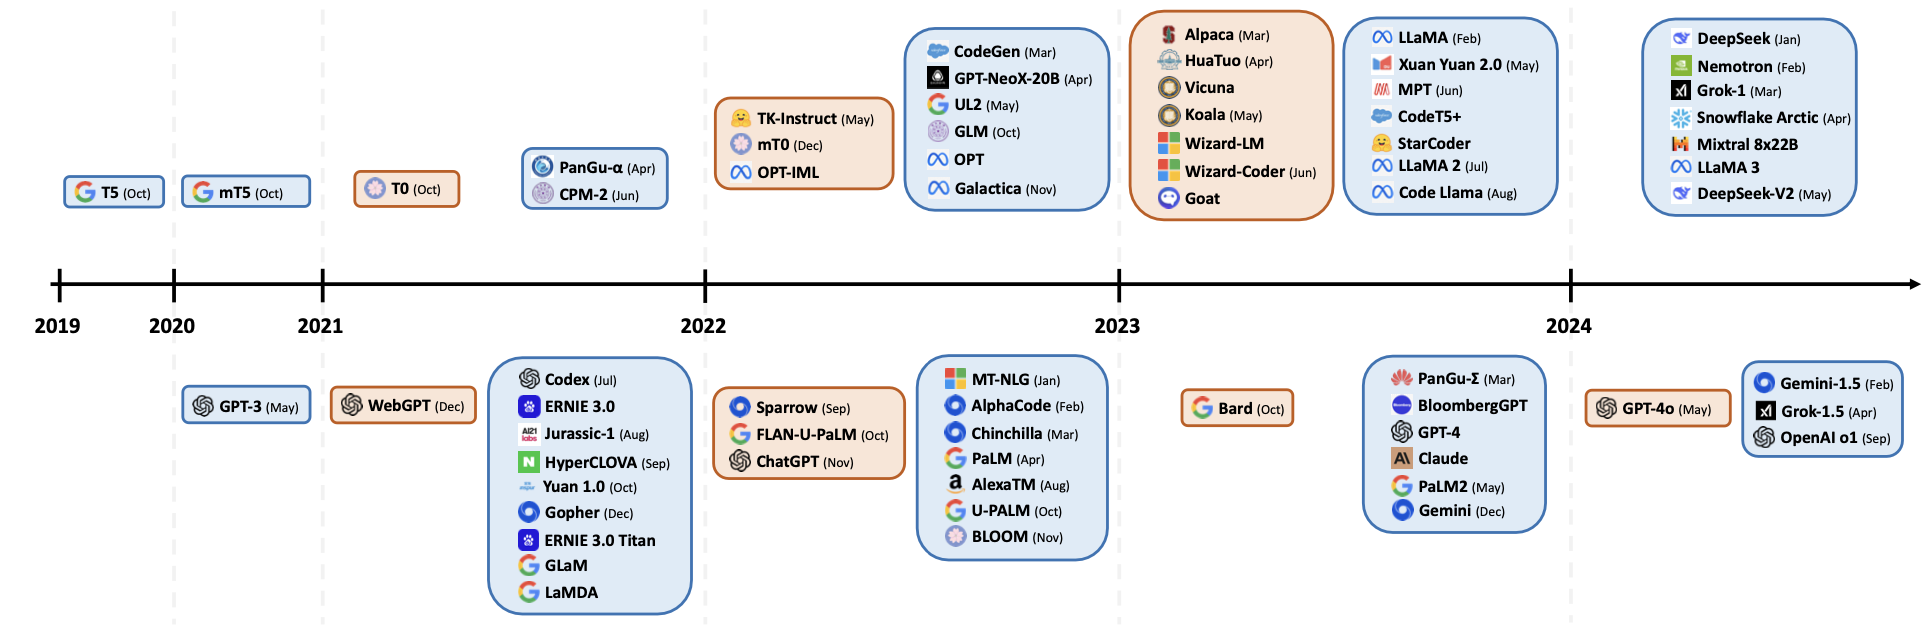
\includegraphics[width=\textwidth]{figures/literature-review/llms-over-the-years.png}
     \rule{35em}{0.5pt}
    \caption{Timeline of \gls{llm} releases: blue cards represent pre-trained models, orange cards denote instruction-tuned models. Open-source models appear on the top, while closed-source models are on the bottom, showing the shift toward open-source and instruction-tuned trends. (\textcite{Naveed2023})}
 \label{fig:llms-over-the-years}
\end{figure}

\glspl{llm}, such as OpenAI's GPT series \cite{Radford2018ImprovingLU}, Google's BERT \cite{Devlin2019BERTPO}, and more recent iterations like GPT-4, are typically built on transformer architectures \cite{Vaswani2017}.
The transformer model introduced a self-attention mechanism that efficiently captures contextual relationships between words across large textual sequences, overcoming limitations of earlier models like \glspl{rnn} and \glspl{lstm} in handling long-range dependencies.
These models are pre-trained on massive corpora containing diverse text from books, articles, and web sources, allowing them to generalize linguistic patterns, syntax, semantics, and even factual knowledge embedded in the data.
According to \textcite{Chang2024}, \glspl{llm} perform a wide range of tasks in \gls{nlp}, often achieving state-of-the-art results across various benchmarks.
Fig.~\ref{fig:llms-overview} provides a broader overview of the organization of \glspl{llm}, categorizing them into seven distinct branches: pre-training, fine-tuning, efficiency, inference, evaluation, applications, and challenges.
These branches reflect the key aspects of the development, deployment, and evaluation of \glspl{llm}.
Pre-training focuses on the foundational step of training models on vast, diverse corpora to learn language representations.
Fine-tuning involves adapting pre-trained models for specific tasks, enhancing their performance on downstream applications.
Efficiency addresses the computational and energy requirements of training and deploying \glspl{llm}, emphasizing methods like parameter-efficient tuning and pruning to reduce resource consumption.
The inference branch examines the process of generating outputs from trained models, focusing on optimizing speed and accuracy.
More advanced capabilities, such as few-shot and zero-shot learning, enable \glspl{llm} to adapt to new tasks with minimal to no task-specific training data, a feature prominently demonstrated by GPT-3 \cite{NEURIPS2020_1457c0d6}.
Evaluation highlights the metrics and benchmarks used to assess \glspl{llm}' performance on various tasks, ensuring they meet quality standards.
Applications span the diverse real-world use cases of \glspl{llm}, from natural language understanding to robotics and multi-modal systems.
Finally, challenges encompass the limitations and issues of \glspl{llm}, including bias, hallucination, and environmental impact, offering directions for future research and improvement.
These branches collectively define the lifecycle and scope of advancements in \glspl{llm} research, providing a comprehensive framework for understanding their capabilities and impact.

\begin{figure}[htbp]
    \centering
 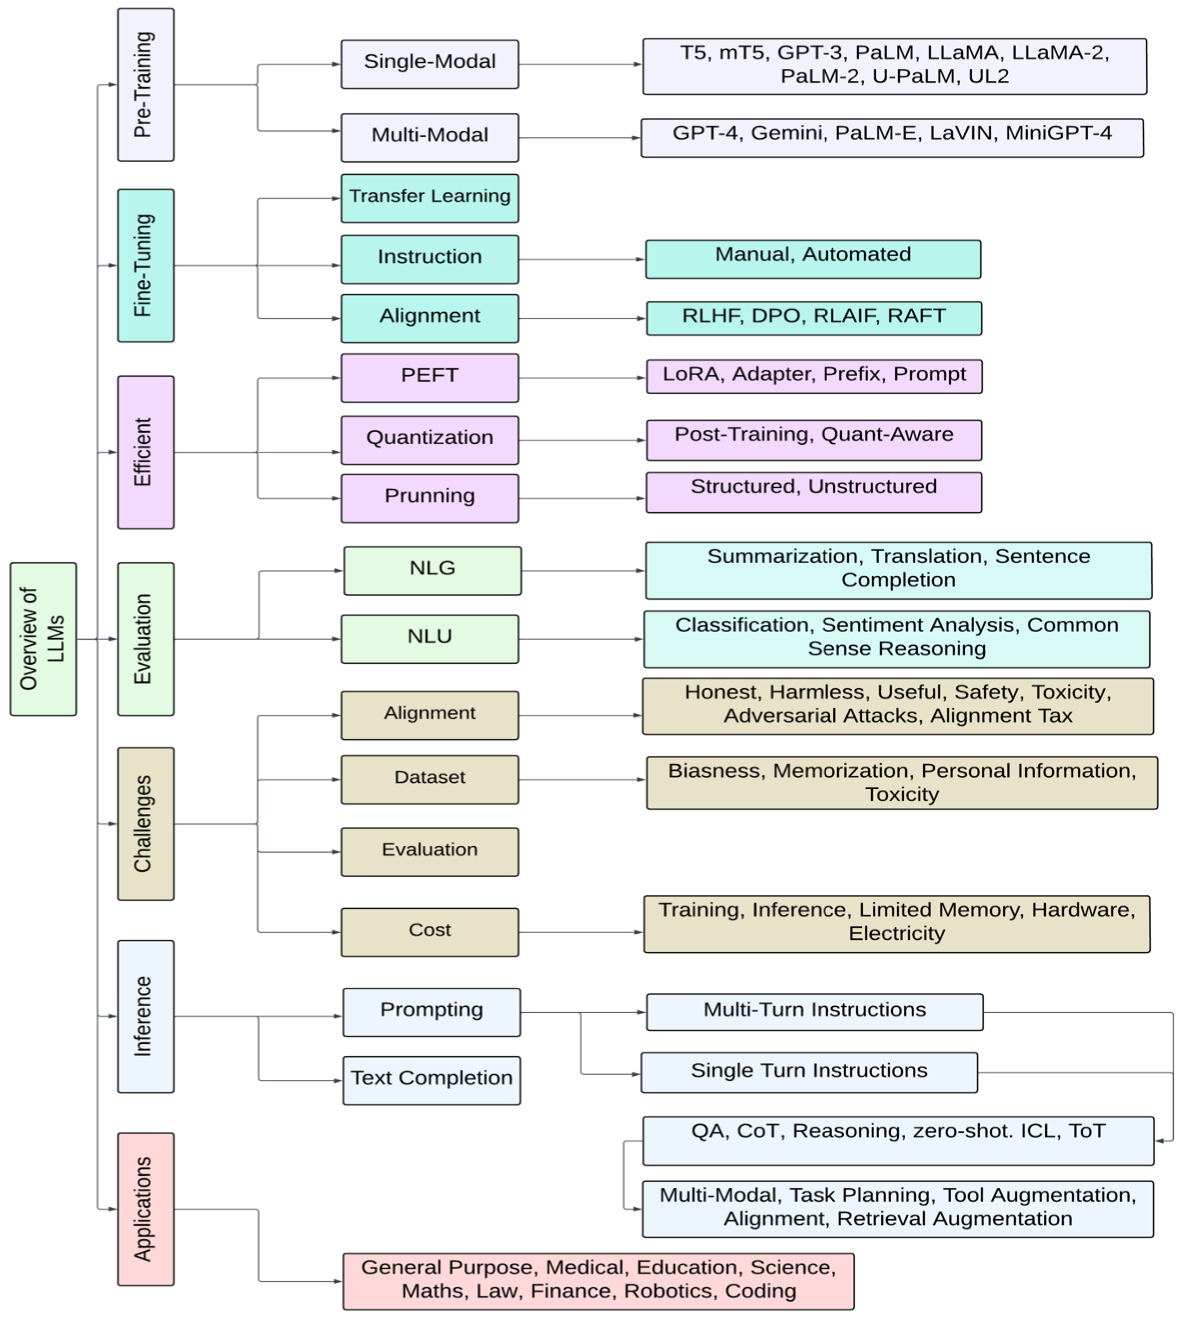
\includegraphics[width=0.8\textwidth]{figures/literature-review/llms-overview.png}
     \rule{35em}{0.5pt}
    \caption{An overview of \glspl{llm} divided into seven branches: pre-training, fine-tuning, efficiency, evaluation, challenges, inference, and applications. (\textcite{Naveed2023})}
 \label{fig:llms-overview}
\end{figure}

This adaptability has made \glspl{llm} suitable for tasks requiring contextual reasoning, dialogue systems, and even code generation, as seen in models like Codex \cite{Chen2021EvaluatingLL}, which powers tools such as GitHub Copilot\footnote{\url{https://github.com/features/copilot}}.
The applications of \glspl{llm} span numerous domains, reflecting their versatility and broad impact.
In industry, \glspl{llm} power conversational agents, customer service bots, and content creation tools.
In research and education, they facilitate automated summarization of scientific literature, personalized tutoring, and question-answering systems to support knowledge discovery.
The integration of \glspl{llm} with domain-specific knowledge graphs and ontologies further enhances their reliability, particularly in specialized areas such as medicine, law, and scientific discovery \cite{Yang2024}.
Despite their strengths, \glspl{llm} have some limitations.
One important problem is their dependence on vast computational resources for training, which has implications for environmental sustainability \cite{Strubell2019EnergyAP}.
Furthermore, \glspl{llm} tend to propagate biases present in the training data, leading to inconsistencies when deployed in real-world applications \cite{Naveed2023}.
They also suffer from factual inaccuracies and hallucinations, where the model generates plausible yet incorrect information \cite{Chang2024}, which limits their applicability in high-stakes environments requiring factual precision.
Moreover, the lack of interpretability in \glspl{llm} remains a significant challenge, as their outputs are generated from complex internal representations that are not easily explainable, leading to questions about trust and accountability \cite{Naveed2023}.
Nevertheless, the advantages of \glspl{llm} are substantial, as they offer unprecedented performance in language-related tasks, significant generalizability, and the ability to operate across diverse applications without extensive task-specific engineering.
In their study, \textcite{Naveed2023} discuss that current research about \glspl{llm} efforts are focused on addressing their limitations, particularly improving energy efficiency, reducing bias, enhancing factual accuracy, and developing methods for better interpretability.
As \glspl{llm} continue to evolve, their integration with structured knowledge systems and advancements in alignment with human intent are likely to redefine their role in solving complex problems across industries.